\subsection{Inference on M2}

\begin{figure}[h]
    \centering
    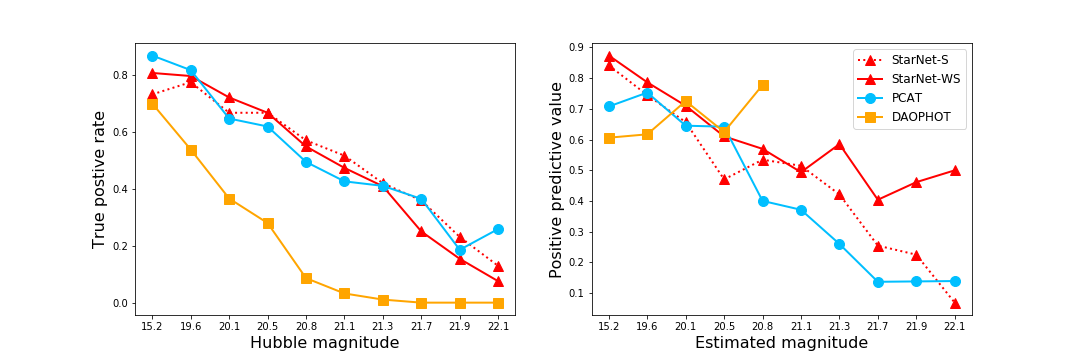
\includegraphics[width=0.99\textwidth]{figures/summary_statistics_m2.png}
    \caption{True positive rate and positive predicted value of various cataloging
    procedures on M2, plotted against magnitude percentile.
    Smaller magnitudes correspond to brighter stars. }
    \label{fig:summary_stats}
\end{figure}

% \begin{table}[!tb]
% \centering
% \caption{Performance metrics on M2.
% For probabilistic methods (StarNet and PCAT)
% the ``\#stars" column refers to the mean number of stars under the (approximate) posterior, while the right-most column displays the 5-th and 95-th percentiles under the posterior. }
% \label{tab:summary_stats}
% \begin{tabular}{l|ccc|cc}
% \toprule
%      Method &   TPR &   PPV &  F1 score &  \#stars & (q-5\%, q-95\%)\\
% \midrule
%     DAOPHOT &  0.20 &  0.63 &      0.30 &     295 & -- \\
%        PCAT &  0.56 &  0.40 &      0.47 &    1672 & (1664, 1680)\\
%  Sleep-only &  0.51 &  0.47 &      0.49 &    1292 & (1260, 1324)\\
%  Wake-sleep &  0.51 &  0.60 &      0.55 &     1014 & (987, 1041)\\
%      %Hubble &  1.00 &  1.00 &      1.00 &     1114 & -- %\\
% \bottomrule
% \end{tabular}
% \end{table}

\begin{table}[!tb]
\centering
\caption{Performance metrics on M2.
For probabilistic methods (StarNet and PCAT)
the ``\#stars" columns provide the mean along with the 5th and 95th percentiles
for the number of stars under the (approximate) posterior,
The number of stars in the Hubble catalog is 1114. }
\label{tab:summary_stats}
\begin{tabular}{l|ccc|cc}
\toprule
& & & & \multicolumn{2}{c}{\#Stars} \\
     Method &   TPR &   PPV &  F1 score &  mean & (q-5\%, q-95\%)\\
\midrule
    DAOPHOT &  0.20 &  0.65 &      0.31 &     357 & -- \\
       PCAT &  0.55 &  0.37 &      0.44 &    1672 & (1664, 1680)\\
 StarNet (our) &  0.53 &  0.48 &      \textbf{0.50} &    1462 & (1430, 1497)\\
\bottomrule
\end{tabular}
\end{table}


\begin{figure}[h]
    \centering
    \vspace{-3cm}
    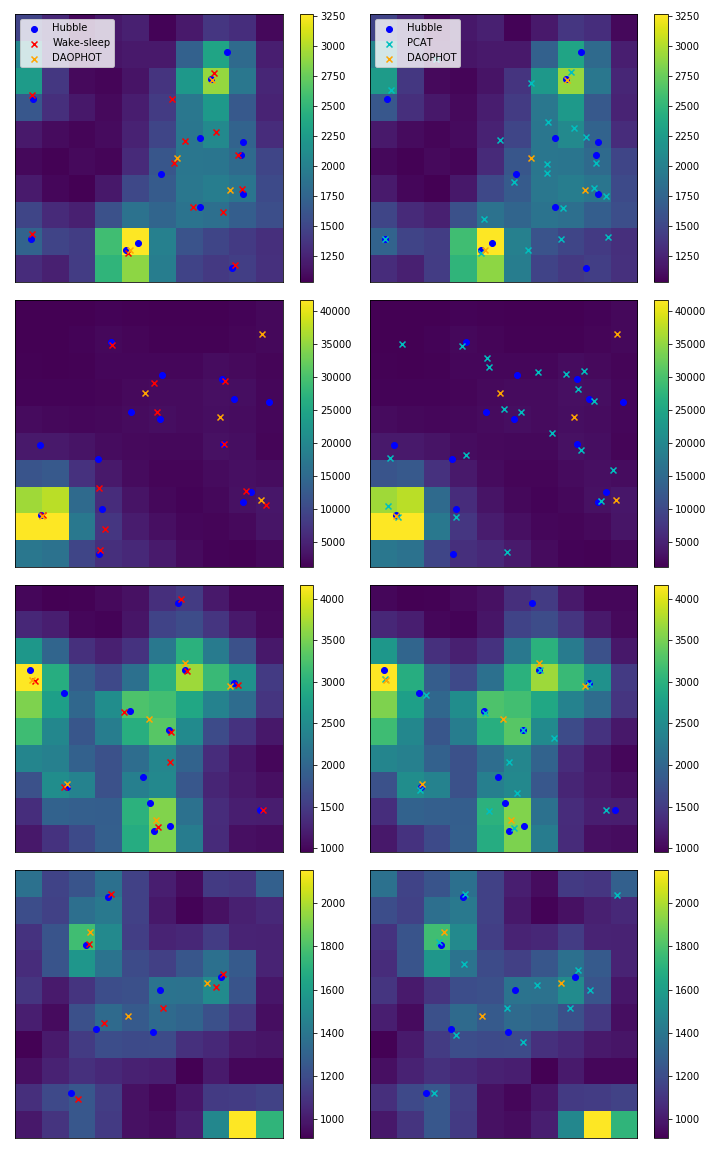
\includegraphics[width=0.8\textwidth]{figures/example_subimages.png}    
    \vspace{-3cm}
    \caption{Estimated catalogs on four 10$\times$10 subimages from 
    M2. Blue dots are Hubble stars brighter than the 22nd magnitude. 
    Starnet, Portillos, and DAOPHOT estimated stars are in 
    red, cyan, and orange x's, respectively. }
    \label{fig:example_subimages}
\end{figure}

\begin{figure}[h]
    \centering
    \vspace{-3cm}
    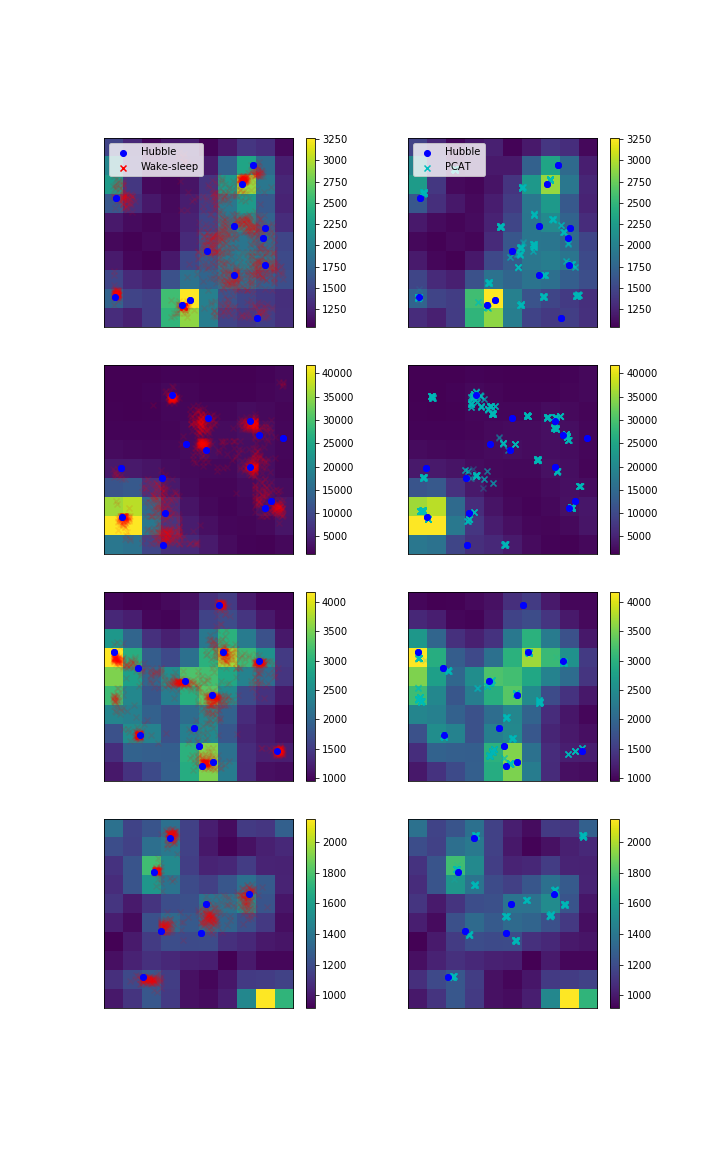
\includegraphics[width=0.8\textwidth]{figures/example_subimages_samples.png}    
    \vspace{-3cm}
    \caption{Four 10$\times$10 subimages from 
    M2. Blue dots are Hubble stars brighter than the 22nd magnitude. 
    We print display the posterior samples from our variational 
    posterior (left) and from the MCMC chain of Portillos (right). }
    \label{fig:example_subimages_sampled}
\end{figure}

\begin{figure}[h]
    \centering
    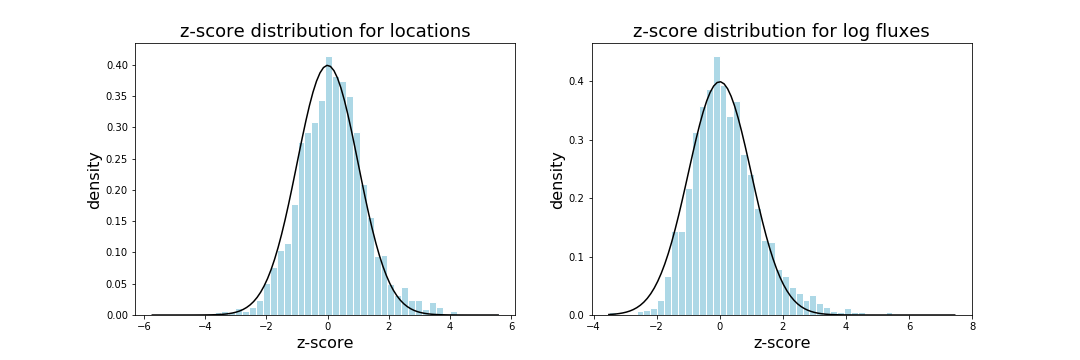
\includegraphics[width=0.99\textwidth]{figures/z-score_calibration.png}    
    \caption{The calibration of uncertainties in our variational posterior. Conditional on the true number of stars, we compute the z-score of the true location or log flux evaluated at our 
    variational posterior. }
    \label{fig:z-score_calibration}
\end{figure}


\begin{figure}[h]
    \centering
    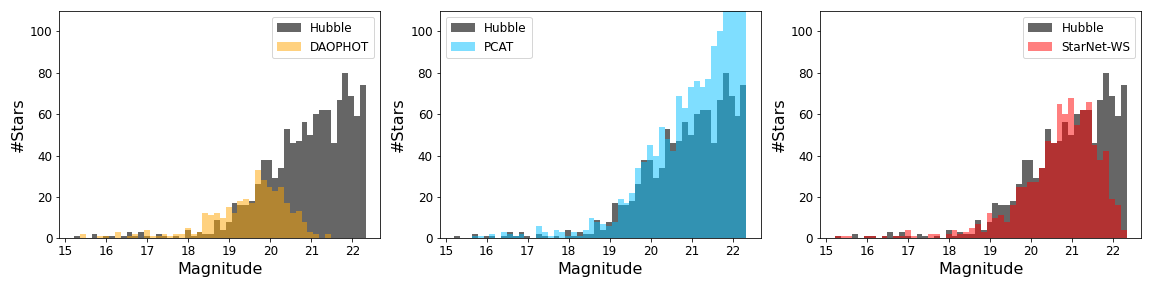
\includegraphics[width=0.99\textwidth]{figures/luminosity_fun.png}
    \caption{Source magnitude histograms on M2. }
    \label{fig:luminosity_fun_m2}
\end{figure}

\begin{figure}[h]
    \centering
    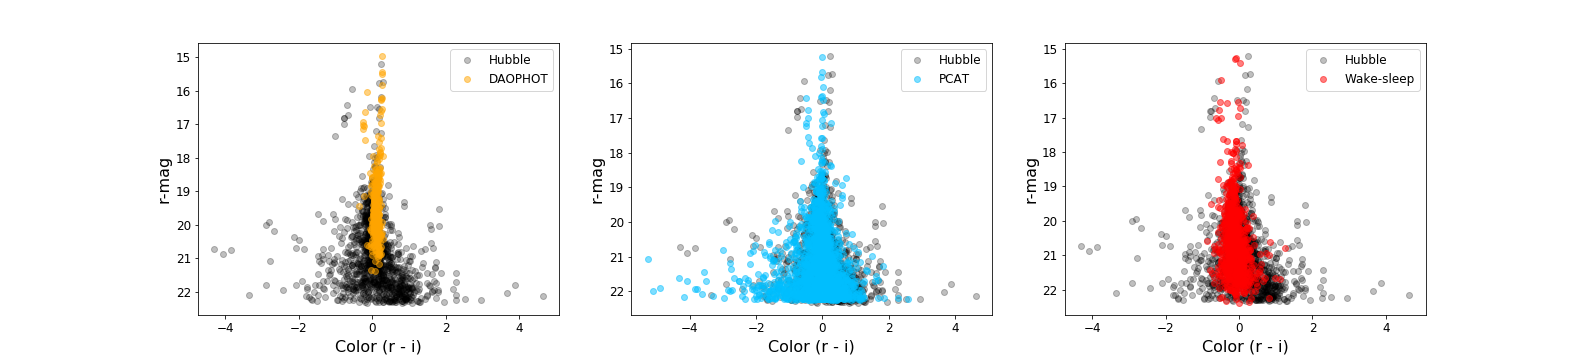
\includegraphics[width=0.99\textwidth]{figures/cmd.png}
    \caption{Color magnitude diagrams on M2. }
    \label{fig:cmd_m2}
\end{figure}


\subsection{Estimation of model parameters}
\input{tables/chi_sq_stats.txt}

\begin{figure}[h]
    \centering
    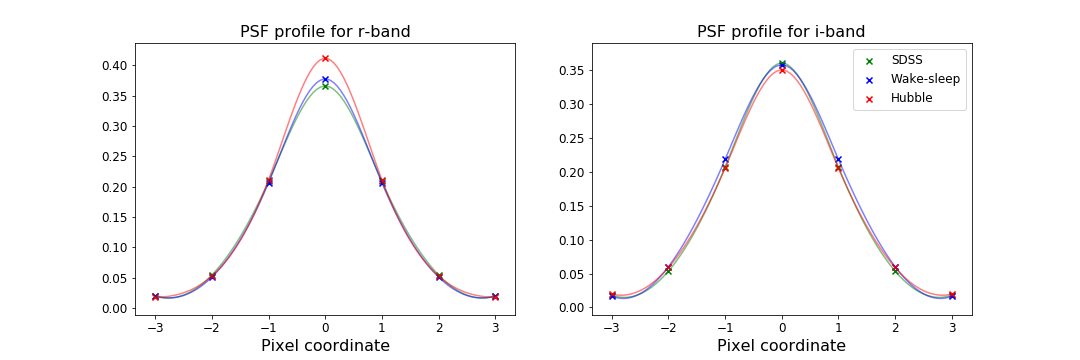
\includegraphics[width=0.99\textwidth]{figures/psf_profiles.png}
    \caption{Estimated versus true PSF profiles on M2. The Hubble PSF was
    obtained by optimizing the likelihood conditioned on locations and fluxes
    from the Hubble catalog. }
    \label{fig:psf_profiles}
\end{figure}


% \multicolumn{1}{p{5cm}}{\raggedleft Chi sq. \\ (with Hubble back.)}
% \caption{
% Chi-squared statistics for SDSS, wake-sleep, and Hubble estimated model parameters.
% The chi-squared statistic is defined as
% $\sum_{bij}\frac{([\text{obs.image}]_{bij} - [\text{recon.image}]_{bij})^2}{[\text{recon.image}]_{bij}}$.
% In the middle column, ``model parameters" refer to both background and PSF.
% In the right column, we fix the background to the Hubble estimate, and examine
% chi-squared statistics as the PSF varies.}
